\documentclass[conference,a4paper]{IEEEtran}
\usepackage[utf8]{inputenc}
\usepackage[T1]{fontenc}
\usepackage[brazil]{babel}
\usepackage{graphicx}
\usepackage{booktabs}
\usepackage{amsmath}
\usepackage{url}
\usepackage[hidelinks]{hyperref}
\usepackage{siunitx}
\sisetup{output-decimal-marker={,}, group-separator={.}}
% \input primitivo: o \input do LaTeX quebra \bottomrule no fim de uma tabela
\makeatletter\newcommand\tabinput[1]{\@@input #1 }\makeatother

\begin{document}

\title{Carrinho de Compras Replicado com\\Relógios Vetoriais e Replicação Epidêmica}

\author{\IEEEauthorblockN{Gustavo Estechea (RA \texttt{XXXXXX}) \quad Lucas (RA \texttt{XXXXXX})}
\IEEEauthorblockA{MC714 -- Sistemas Distribuídos, 2º semestre de 2026, IC/Unicamp\\
Repositório: \url{https://gitlab.ic.unicamp.br/XXXX/mc714-trabalho2}\\
Vídeo: \url{https://XXXX}}}

\maketitle

\begin{abstract}
Neste trabalho implementamos, em Go e usando só a biblioteca padrão, dois
algoritmos que se complementam: relógios vetoriais com entrega causal e
replicação epidêmica por anti-entropia. Com eles montamos um carrinho de
compras replicado em $N$ nós, cada um no seu contêiner, que aceita escritas em
qualquer nó e volta a um estado comum depois de partições e reinícios. A
correção é verificada por testes automatizados e por um script que confere o
estado final de cada experimento. Medimos convergência, mensagens, latência e o
tamanho do relógio vetorial variando número de nós, intervalo de gossip, carga
e atraso de rede.
\end{abstract}

\section{Motivação e visão geral}
Um carrinho de compras precisa continuar aceitando itens mesmo quando parte do
sistema está fora do ar. Por isso preferimos disponibilidade a consistência
forte e adotamos um modelo multi-líder: qualquer nó aceita \texttt{ADD} e
\texttt{REMOVE} na hora e repassa a operação depois.

Esse modelo traz dois problemas. Primeiro, operações relacionadas precisam ser
aplicadas na ordem certa, e operações concorrentes precisam ser reconhecidas
como tal; é para isso que usamos relógios vetoriais~\cite{mattern88,fidge88},
que estendem os relógios lógicos de Lamport~\cite{lamport78} e conseguem
distinguir concorrência de causalidade~\cite{vansteen23}.
Segundo, toda operação tem que chegar a todas as réplicas, o que resolvemos com
anti-entropia epidêmica~\cite{demers87}. Os dois algoritmos não ficam
isolados: o relógio vetorial de cada réplica é exatamente o resumo que ela
manda na anti-entropia para descobrir o que falta a cada lado.

\section{Arquitetura}
Todos os nós rodam o mesmo binário (\texttt{cmd/node}), cada um em um
contêiner próprio, configurado apenas por variáveis de ambiente do
\texttt{compose.yaml}. A comunicação é HTTP/JSON pela rede \emph{bridge}
\texttt{gossip-net}, e cada nó encontra os outros pelo nome
(\texttt{node-k}) via DNS do Compose. O código está dividido em
\texttt{clock} (relógio vetorial), \texttt{cart} (réplica e entrega causal),
\texttt{replication} (rodadas de anti-entropia e monitor de vizinhos),
\texttt{transport} (servidor e cliente HTTP), \texttt{topology},
\texttt{metrics} e \texttt{node}. Não reaproveitamos código de terceiros.

A topologia é fixa e igual em todos os nós: uma cadeia
$\texttt{node-1}-\dots-\texttt{node-}N$, que garante que o grafo seja conexo,
mais uma aresta extra sorteada com semente fixa (\texttt{TOPOLOGY\_SEED}=42)
para encurtar o diâmetro. Um nó recusa (HTTP 403) gossip de quem não é seu
vizinho.

Cada vez que um nó sobe ele vira uma nova \emph{encarnação}, com
identificador \texttt{node-k@<nanossegundos do boot>}. As operações recebem o
ID \texttt{<encarnação>:<contador>} e cada unidade adicionada recebe
\texttt{<op>/<i>}. Com isso, um nó reiniciado nunca reutiliza um ID antigo.

Sobre a semântica do carrinho: \texttt{ADD(p,q)} cria $q$ unidades do produto
$p$, e \texttt{REMOVE(p,q)} marca como removidas (\emph{tombstones}) as $q$
menores unidades vivas de $p$ que a origem conhecia, listando-as na própria
operação. Se não houver unidades suficientes, a resposta é 409. A quantidade
de um produto é o número de unidades vivas. Na prática isso é um conjunto
\emph{observed-remove} em que a adição vence~\cite{shapiro11}: uma unidade
adicionada ao mesmo tempo que um \texttt{REMOVE} acontece em outro nó não é
afetada por ele.

\section{Algoritmo 1: relógios vetoriais e entrega causal}
\subsection{Funcionamento}
Cada réplica $i$ guarda um vetor $V_i$ que associa cada encarnação a um
contador; uma chave ausente vale 0. Ao criar uma operação local, a réplica
incrementa $V_i[i]$ e anexa uma cópia de $V_i$ à operação. Ao aplicar uma
operação $m$, faz $V_i \gets \max(V_i, V_m)$ entrada a entrada. Dizemos que
$V_a < V_b$ quando $V_a \le V_b$ em todas as entradas e os vetores são
diferentes; se nenhum dos dois é menor que o outro, as operações são
concorrentes.

Uma operação $m$ vinda da origem $j$ só é aplicada quando
\begin{equation}
V_m[j] = V_i[j]+1 \quad\text{e}\quad V_m[k]\le V_i[k]\ \ \forall k\ne j,
\end{equation}
ou seja, quando ela é a próxima de $j$ e a réplica já viu tudo o que $j$ tinha
visto. Até lá ela espera em um buffer. Se $V_m[j]\le V_i[j]$, ou se ela já
está no buffer, é uma duplicata e é descartada. Um \texttt{REMOVE} ainda passa
por mais uma checagem: cada unidade removida precisa vir de um \texttt{ADD}
cujo relógio seja $\le V_m$, isto é, a origem precisava conhecer aquela
unidade. Se não for o caso, a operação é rejeitada. Quando uma operação é
concorrente com a última aplicada no mesmo produto, o nó registra o evento
\texttt{concurrent\_ops\_detected}.

\subsection{Modelo do sistema}
Assumimos um sistema assíncrono. A entrega causal não depende de tempo
nenhum: ela espera o quanto for preciso pelos predecessores. Os canais podem
perder, duplicar e reordenar mensagens, e não supomos FIFO; o buffer resolve a
reordenação e o descarte por contador resolve a duplicação (a perda fica a
cargo da anti-entropia). Consideramos falhas do tipo crash-recovery sem
persistência: um nó que reinicia volta com relógio vazio, como uma encarnação
nova, e por isso ganha uma entrada nova no vetor. Não tratamos falhas
bizantinas; lotes malformados são recusados por inteiro, mas um nó mal
intencionado poderia mentir no próprio relógio. Relógios físicos não são
usados para ordenar nada; o horário do boot serve só para distinguir
encarnações.

\subsection{Propriedades}
Uma execução correta satisfaz, como segurança: (S1) nenhuma operação é
aplicada antes de seus predecessores causais; (S2) cada operação é aplicada no
máximo uma vez; (S3) os contadores de cada origem aparecem sem lacunas;
(S4) um \texttt{REMOVE} só remove unidades que sua origem observou; (S5)
operações pendentes não aparecem nas quantidades, que portanto nunca ficam
negativas. Como vivacidade: (L1) se os predecessores de uma operação chegam em
algum momento, ela também é aplicada.

\subsection{Custo}
Comparar e mesclar relógios custa $O(E)$, onde $E$ é o número de entradas do
vetor, e cada operação carrega $O(E)$ bytes de metadados. Sem falhas,
$E = N$. Como não há coleta de lixo, cada reinício acrescenta uma entrada que
nunca sai.

\section{Algoritmo 2: anti-entropia epidêmica}
\subsection{Funcionamento}
A cada \texttt{GOSSIP\_INTERVAL}, cada nó $i$ conversa em paralelo com cada
vizinho $P$ em duas etapas. Na primeira (\emph{pull}), $i$ envia $V_i$ e $P$
devolve $V_P$ junto com as operações que $i$ ainda não tem, que são as $m$ do
log de $P$ com $V_m[\text{orig}(m)] > V_i[\text{orig}(m)]$; $i$ aplica essas
operações pela entrega causal. Na segunda (\emph{push}), $i$ usa $V_P$ para
calcular o que falta a $P$ e envia, se houver algo. Nenhum estado é
sobrescrito; tudo passa pelo mesmo \emph{merge}.

Cada nó também mantém um contador de falhas consecutivas por vizinho. Ao
chegar em três (\texttt{FAILURE\_THRESHOLD}), ele registra
\texttt{gossip\_peer\_unreachable}. Esse monitor serve só para observação e
não muda o comportamento do protocolo.

\subsection{Modelo do sistema}
A segurança não depende de tempo. Para a vivacidade precisamos de um pouco de
sincronia: depois que a rede se recupera, as mensagens entre vizinhos têm que
chegar antes do \emph{timeout}, que é explícito em toda requisição
(\texttt{HTTP\_TIMEOUT}=2\,s). Os canais são HTTP sobre TCP. Uma troca perdida
é simplesmente refeita na rodada seguinte, e receber a mesma operação duas
vezes não tem efeito (S2). Tratamos crash-recovery sem persistência e
partições de rede. Uma limitação que aceitamos: se um nó cai antes de repassar
uma operação, ela se perde.

\subsection{Propriedades}
Segurança: (S6) o estado só cresce por \emph{merge}; (S7) um lote com qualquer
operação inválida não altera nada. Vivacidade: (L2) se as escritas param e os
nós vivos formam um grafo conexo, todas as réplicas chegam ao mesmo log,
relógio e quantidades; (L3) um nó reiniciado recupera toda operação que algum
vizinho alcançável ainda tenha; (L4) depois que uma partição é desfeita, os
dois lados convergem.

\subsection{Custo}
Em cada rodada um nó faz uma troca por vizinho, com uma ou duas mensagens.
Cada troca carrega o relógio, de tamanho $O(E)$, mais as operações que
faltam. Uma operação leva no máximo $D$ rodadas para chegar a todos, sendo $D$
o diâmetro do grafo, então esperamos convergência em torno de
$D\cdot\texttt{GOSSIP\_INTERVAL}$. Com a cadeia mais uma aresta, $D\le N-1$.

\section{Verificação da correção}
Os testes automatizados (\texttt{go test ./...}, também com \texttt{-race})
cobrem o relógio vetorial (ordem, \emph{merge}, ausência de efeitos
colaterais) e vários casos da entrega causal: \texttt{REMOVE} que chega antes
do \texttt{ADD} fica no buffer, lacuna de contador fica no buffer, reaplicar é
inofensivo, um lote inválido não muda nada, remover unidade não observada é
rejeitado, \texttt{ADD} concorrente sobrevive ao \texttt{REMOVE} e dois
\texttt{REMOVE}s concorrentes colapsam. Há também um teste aleatorizado de
convergência e testes de integração com vários nós em processo (cadeia, push
duplicado, concorrência, reinício, vizinho fora do ar, topologia aleatória).
O teste ponta a ponta (\texttt{just e2e}) sobe quatro contêineres de verdade e
passa por propagação, partição e reinício.

Além disso, ao fim de cada experimento o script \texttt{verify.py} lê o
estado completo de cada nó (\texttt{/debug/state}, que inclui o log de
operações) e confere: contadores contíguos por origem (S3); todo predecessor
causal aparece antes no log (S1); \texttt{REMOVE}s só sobre unidades
observadas (S4); quantidades recalculadas a partir do log batem com as
reportadas; nenhuma operação pendente; e todos os nós iguais (L2--L4).
Nas 71 execuções da Seção~\ref{sec:res}, inclusive as com partição e reinício,
todas essas verificações passaram e nenhum \texttt{REMOVE} foi rejeitado.

\section{Metodologia experimental}
\subsection{Ambiente}
Rodamos tudo em uma única máquina: Intel Core i5-13450HX (16 \emph{threads}),
16\,GB de RAM, Ubuntu 22.04.5 com kernel 6.1.0-1013-oem, Docker 29.8.2,
Compose v5.6.0, Go 1.26.1 e Python 3.10.12. Vale lembrar que contêineres na
mesma máquina são nós lógicos, mas não falham de forma independente:
dividem CPU, kernel e uma rede local quase sem latência. Por isso os tempos
medidos são otimistas em relação a uma implantação real.

\subsection{Procedimento}
O script \texttt{run.py} gera um \texttt{compose.yaml} com $N$ nós, sobe o
cluster e dispara o gerador de carga (\texttt{cmd/loadgen}, com semente
registrada e \emph{timeout} de 2\,s por requisição). Em seguida injeta a falha,
se houver, consulta \texttt{/debug/metrics} a cada 200\,ms até o cluster
convergir, salva CSV, JSON e logs brutos e roda o \texttt{verify.py}. A carga
tem taxa constante, é distribuída entre os nós e usa 50 produtos, 20\% de
\texttt{REMOVE} e estoque inicial de 1000 unidades por produto. Cada execução
tem 10\,s de aquecimento, descartados, e 60\,s medidos. Repetimos cada
configuração cinco vezes com sementes diferentes e reportamos média com
intervalo de confiança de 95\% ($1{,}96\,s/\sqrt{n}$), além de percentis.

\subsection{Métricas}
Para a replicação, a métrica principal é o \emph{tempo de convergência}:
quanto tempo passa entre o fim da carga (ou a cura da falha) e o momento em
que todos os nós têm o mesmo relógio, o mesmo número de operações, as mesmas
quantidades e nenhuma pendência. Ela mede diretamente L2--L4. Também medimos
\emph{mensagens por operação}, que mostra o custo de disseminação, e a
\emph{latência de escrita} percebida pelo cliente (p50, p95 e p99, só das
respostas 201). Para o relógio vetorial, medimos o seu \emph{tamanho}: o
número de entradas $E$, os bytes do relógio em cada operação e a fração dos
bytes de cada operação que vai para ele. Isso mostra quanto de metadado o
Algoritmo~1 acrescenta. Nos cenários de falha medimos ainda o \emph{tempo de
detecção}, da falha até algum vizinho marcar o nó como inalcançável.

\subsection{Parâmetros}
Variamos um parâmetro por vez, sempre em três níveis: número de nós
($N=4,6,8$); intervalo de gossip (250\,ms, 1\,s e 4\,s); carga (5, 20 e 50
ops/s); e latência injetada com Toxiproxy em todos os enlaces de gossip (0, 50
e 150\,ms, com 10\,ms de \emph{jitter}). Fora o parâmetro variado, usamos
$N=6$, intervalo de 1\,s e 20 ops/s. Nos cenários de falha, com $N=6$, o nó 3
é desconectado da rede (partição) ou parado (\texttt{docker compose stop})
aos 20\,s, e reconectado ou religado aos 40\,s.

\subsection{Dados e reprodução}
Todos os dados brutos estão no repositório~\cite{dados}, em
\texttt{project2/infrastructure/experiments/results/}, uma pasta por execução
(\texttt{<data UTC>-<nome>}). Cada pasta guarda o \texttt{compose.yaml}
gerado, uma linha por requisição do cliente (\texttt{requests.csv}: nó, tipo,
status, latência e horários), o resumo da carga, as métricas finais
(\texttt{metrics-node-k.json}) e o estado completo de cada nó
(\texttt{state-node-k.json}, com o log de operações), os logs do cluster com
horário, o resultado do \texttt{verify.py} e um \texttt{summary.json} com a
configuração, as sementes, os instantes da falha, a convergência e os dados
da máquina. O \texttt{analyze.py} consolida tudo em
\texttt{experiments/analysis/runs.csv} (uma linha por execução) e
\texttt{aggregate.csv} (média e IC por configuração), e o
\texttt{report/figuras.py} gera as tabelas e figuras deste relatório a partir
do \texttt{runs.csv}. Para refazer tudo, a partir de
\texttt{project2/infrastructure}: \texttt{just exp-all}, \texttt{just
analyze} e \texttt{python3 ../report/figuras.py}. Os valores absolutos
dependem da máquina; as tendências são o que esperamos reproduzir.

\section{Resultados}\label{sec:res}
\begin{table*}[t]
\centering
\caption{Média $\pm$ IC 95\% de 5 execuções por configuração. Conv.: tempo de
convergência; msg/op: mensagens de gossip por operação do cliente; p99:
latência de escrita; $E$: entradas do relógio vetorial; B/op: bytes do relógio
em cada operação; \%op: fração dos bytes da operação ocupada pelo relógio;
ok: execuções que convergiram e passaram no \texttt{verify.py}. Fonte:
\texttt{experiments/results/}~\cite{dados}.}
\label{tab:res}
\begin{tabular}{lrrrrrrr}
\toprule
Configuração & Conv. (s) & msg/op & p99 (ms) & $E$ & B/op & \%op & ok \\
\midrule
\tabinput{figs/tabela.tex}
\bottomrule
\end{tabular}
\end{table*}

A Tabela~\ref{tab:res} resume as 71 execuções (70 da matriz mais um teste
rápido); os valores por execução estão em \texttt{runs.csv}~\cite{dados}.
Todas convergiram e todas passaram na verificação de estado.

\subsection{Número de nós}
\begin{figure}[t]
\centering
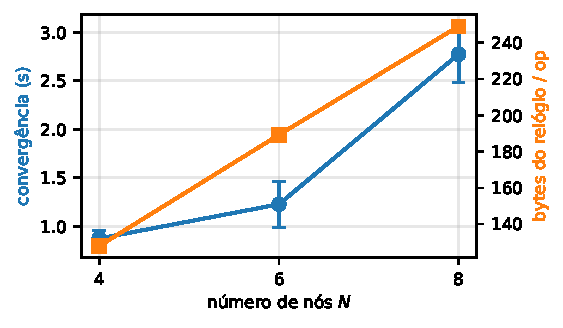
\includegraphics[width=\columnwidth]{figs/nos.pdf}
\caption{Convergência (azul) e bytes do relógio vetorial por operação
(laranja) em função de $N$. Barras: IC 95\%.}
\label{fig:nos}
\end{figure}
A Fig.~\ref{fig:nos} mostra que a convergência passou de 0,87\,s ($N=4$) para
1,23\,s ($N=6$) e 2,77\,s ($N=8$). O salto entre 6 e 8 não é só efeito de
$N$: pelos logs (\texttt{configured\_neighbors}), com a semente 42 a aresta
extra fecha um anel para $N=4$ e $N=6$ (diâmetro $D=2$ e $3$), mas para $N=8$
ela liga \texttt{node-1} a \texttt{node-3} e o grafo continua quase uma
cadeia, com $D=6$. Dividindo a convergência por $D\cdot T$ ($T=1$\,s)
obtemos 0,43, 0,41 e 0,46, ou seja, ela cresce linearmente com o diâmetro,
como previsto. O fator fica abaixo de 1 porque as rodadas dos nós não são
sincronizadas e uma operação pode andar mais de um salto por intervalo (um nó
pode fazer \emph{pull} e logo depois ser alvo do \emph{push} de outro).

Já o relógio vetorial cresce com $N$ e não com $D$: $E=N$ em todas as
execuções sem falha, e os bytes do relógio por operação foram 128, 189 e 249,
cerca de 31 bytes por entrada (a chave \texttt{node-k@<19 dígitos>} domina).
Isso é 42\%, 51\% e 58\% de cada operação, que tem uns 370 bytes em JSON.
Para um carrinho com poucos itens por operação, o relógio já é o maior
componente da mensagem, e o custo $O(N)$ por operação seria o primeiro
problema a escalar.

\subsection{Intervalo de gossip}
\begin{figure}[t]
\centering
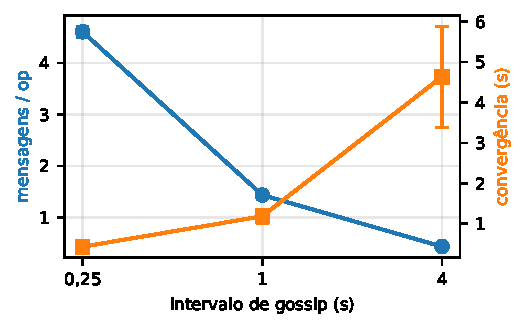
\includegraphics[width=\columnwidth]{figs/intervalo.pdf}
\caption{Mensagens por operação (azul) e convergência (laranja) para
intervalos de 0,25, 1 e 4\,s, $N=6$. Eixo $x$ em escala log.}
\label{fig:int}
\end{figure}
Aqui aparece o compromisso clássico da anti-entropia (Fig.~\ref{fig:int}).
Com o intervalo 16 vezes maior (0,25\,s $\to$ 4\,s), as mensagens por operação
caem de 4,6 para 0,4 e a convergência sobe de 0,43\,s para 4,64\,s. As duas
grandezas variam quase proporcionalmente ao intervalo, porque o número de
trocas por segundo é fixo ($N\cdot\deg/T$) e a convergência é
$\approx 0{,}4\,D\,T$. O tamanho do relógio não muda com o intervalo.

\subsection{Carga}
\begin{figure}[t]
\centering
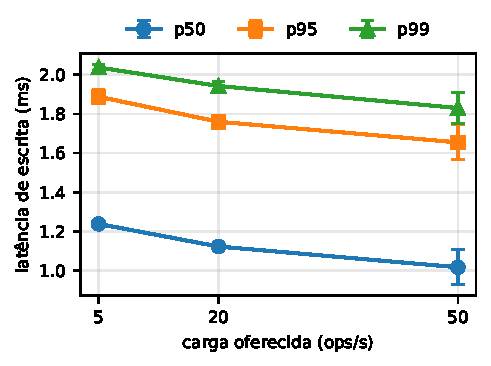
\includegraphics[width=\columnwidth]{figs/carga.pdf}
\caption{Percentis de latência de escrita vistos pelo cliente em função da
carga, $N=6$.}
\label{fig:carga}
\end{figure}
A latência de escrita ficou abaixo de 2,3\,ms no p99 em todas as cargas
(Fig.~\ref{fig:carga}), e até caiu um pouco com mais carga, provavelmente
por efeito de cache e de CPU já ``acordada''. Isso é esperado: a escrita é
aplicada localmente e respondida na hora, sem esperar nenhum outro nó; a
replicação acontece depois, em segundo plano. Com a carga, o custo de
mensagens por operação cai (4,9 $\to$ 1,4 $\to$ 0,6) porque as rodadas
acontecem de qualquer jeito e são amortizadas por mais operações. Os bytes
de gossip por operação também caem, de 2146 para 1485 e 1377, mas bem menos:
o relógio enviado em cada \emph{pull} é amortizado, porém cada operação
continua atravessando todos os enlaces do grafo. A convergência ficou em
torno de 1,1--1,3\,s nos três níveis. Já o número de operações concorrentes
detectadas pelo relógio vetorial cresceu bastante com a carga (68, 1138 e
5794 por execução, em média), sem nenhuma rejeição.

\subsection{Atraso de rede}
Com Toxiproxy acrescentando 50 ou 150\,ms (mais 10\,ms de \emph{jitter}) às
respostas de todo enlace de gossip, a convergência foi 1,15, 1,15 e 1,23\,s
para 0, 50 e 150\,ms; as diferenças ficam dentro do IC. Uma troca completa
(\emph{pull} + \emph{push}) leva no máximo $2\times150$\,ms, bem menos que o
intervalo de 1\,s, então o atraso só desloca um pouco o momento em que cada
salto termina. Esperamos que o efeito apareça quando o atraso se aproximar do
intervalo ou do \emph{timeout} de 2\,s, o que não testamos. A latência do
cliente não muda, pelo mesmo motivo da subseção anterior.

\subsection{Falhas}
\begin{table}[t]
\centering
\caption{Cenários de falha ($N=6$, nó 3, 5 execuções): tempo até algum
vizinho marcar o nó como inalcançável, tempo de recuperação após a
cura/religamento e o pior caso de recuperação. Fonte: execuções
\texttt{failure-*} em~\cite{dados}.}
\label{tab:falhas}
\begin{tabular}{lrrr}
\toprule
Falha & Detecção (s) & Recup. (s) & máx. (s) \\
\midrule
\tabinput{figs/falhas.tex}
\bottomrule
\end{tabular}
\end{table}
A Tabela~\ref{tab:falhas} mostra os dois cenários de falha. Na
\emph{partição}, o nó 3 é desconectado da rede do Compose. Ele mantém seu
estado, mas fica inacessível tanto para os vizinhos quanto para o cliente,
porque a porta publicada passa pela mesma rede; nesse intervalo o restante
do cluster continua recebendo escritas. Depois da reconexão, todos voltaram a
um estado único em 1,27\,s em média (pior caso 1,69\,s), o que confirma L4.
O caso com escritas dos dois lados da partição é coberto pelo teste ponta a
ponta, que isola \texttt{node-1} parando \texttt{node-2} na cadeia e verifica
que as operações não atravessam a partição e depois convergem. No
\emph{reinício}, o nó 3 voltou como uma encarnação nova, sem nada em memória,
e recuperou dos vizinhos o log inteiro (cerca de 1380 operações, uns 720\,kB
em JSON) em 1,06\,s em média, o que confirma L3. Em ambos os cenários, entre
58 e 85 requisições do cliente ao nó 3 falharam por execução, como esperado,
já que o gerador de carga não troca de nó.

O tempo de detecção depende de três falhas consecutivas
(\texttt{FAILURE\_THRESHOLD}). No reinício, a conexão é recusada na hora e
três rodadas de 1\,s dão os 2,4\,s observados. Na partição, os pacotes
simplesmente somem e cada tentativa só falha ao estourar o \emph{timeout} de
2\,s, o que explica os 3,2\,s.

O reinício também mostra o custo do relógio: o nó religado ganha uma
entrada nova e $E$ passa de 6 para 7 em todas as execuções; os bytes de
relógio por operação sobem de 189 para 202. Como não há coleta de lixo, cada
reinício deixa uma entrada permanente.

\section{Limitações}
Não há persistência, então uma operação que ainda não saiu do nó se perde se
ele cair. Tombstones, log e entradas do relógio nunca são removidos, de modo
que memória e metadados só crescem, principalmente quando há reinícios. A
topologia é estática e não há entrada ou saída dinâmica de nós. O detector de
falhas apenas registra o problema. Por fim, todos os números vêm de uma única
máquina, e o harness com Toxiproxy suporta no máximo nove nós.

\section{Conclusões}
Os dois algoritmos funcionaram juntos como esperado. A entrega causal com
relógios vetoriais garantiu, em todas as 71 execuções, que nenhuma operação
fosse aplicada fora de ordem ou duas vezes, e a anti-entropia levou todas as
réplicas ao mesmo estado tanto em operação normal quanto depois de partições e
reinícios. Os números seguem o que a análise previa: a convergência cresce
com o diâmetro do grafo e com o intervalo de gossip
($\approx 0{,}4\,D\,T$), as mensagens por operação caem quando o intervalo ou
a carga sobem, e a latência do cliente não depende da replicação porque a
escrita é local. O custo que mais chama atenção é o do relógio vetorial:
ele cresce com o número de encarnações e já ocupa mais da metade de cada
operação com seis nós. Uma continuação natural seria persistir o estado (para
não criar uma entrada nova a cada reinício), coletar entradas e tombstones
antigos, e trocar o relógio por operação por algo mais compacto, como
\emph{dotted version vectors}.

\begin{thebibliography}{9}
\bibitem{vansteen23} M. van Steen and A. S. Tanenbaum, \emph{Distributed Systems}, 4th ed., distributed-systems.net, 2023.
\bibitem{demers87} A. Demers \emph{et al.}, ``Epidemic algorithms for replicated database maintenance,'' in \emph{Proc. ACM PODC}, 1987, pp. 1--12.
\bibitem{mattern88} F. Mattern, ``Virtual time and global states of distributed systems,'' in \emph{Parallel and Distributed Algorithms}, 1988, pp. 215--226.
\bibitem{fidge88} C. J. Fidge, ``Timestamps in message-passing systems that preserve the partial ordering,'' in \emph{Proc. 11th Australian Computer Science Conf.}, 1988, pp. 56--66.
\bibitem{lamport78} L. Lamport, ``Time, clocks, and the ordering of events in a distributed system,'' \emph{Commun. ACM}, vol. 21, no. 7, pp. 558--565, 1978.
\bibitem{dados} G. Estechea e Lucas, ``Código, dados brutos e scripts dos experimentos do Trabalho 2 de MC714,'' repositório GitLab, tag \texttt{XXXX}, 2026. [Online]. Disponível: \url{https://gitlab.ic.unicamp.br/XXXX/mc714-trabalho2}, diretório \texttt{project2/infrastructure/experiments/}.
\bibitem{shapiro11} M. Shapiro, N. Preguiça, C. Baquero, and M. Zawirski, ``Conflict-free replicated data types,'' in \emph{Proc. SSS}, 2011, pp. 386--400.
\end{thebibliography}

\end{document}
